\noindent \textit{Eagleson's Law: Any code of your own that you haven't looked at for six or more months, might as well have been written by someone else.}

\subsection{A task-based approach}

Many people create a project directory containing a distinct folders for each type of file in the project, like \texttt{raw}, \texttt{code}, and \texttt{data}.
I no longer believe this is a helpful approach.
Viewing a series of files in the \texttt{code} folder and a series of files in the \texttt{data} folder doesn't really make the relationships between them clear.
One tries to list inputs and outputs at the top of each code file,
but one inevitably fails to reliably update the metadata of each code file to accurately describe the inputs it relies upon and the outputs it produces.
And in a team environment, one inevitably has to go back and partition the files into natural chunks of labor that can be divided among collaborators.

We take a task-based approach to organizing our research project.
The key idea: \href{https://hrdag.org/2016/06/14/the-task-is-a-quantum-of-workflow/}{the task is a quantum of workflow}. 
Each task is a separate folder with three subfolders: \texttt{input}, \texttt{code}, and \texttt{output}.
One task's input is another task's output.
I was initially persuaded of the merits of this approach by Patrick Ball's \href{https://www.youtube.com/watch?v=ZSunU9GQdcI}{principled data processing} presentation.
The key part of the talk starts at \href{https://youtu.be/ZSunU9GQdcI?t=15m50s}{15:50}.

This approach has a number of advantages.
One is that the project structure is self-documenting.
You don't have to update the metadata at the top of the code because the input and output directories make the relationships obvious.
In fact, these relationships between tasks can be automatically audited, 
as we show in the next section.
Second, this structure makes the project modular.
A team member can jump in and work on one task in isolation because she/he can take the inputs as given and focus on the task-specific code without having to navigate the rest of the project.
Both of these advantages are also relevant when you return to a project after not looking at it for twelve months.

Some folks dislike the ``quantum'' nature of the task-based approach,
because a research project involves many tasks and thus this approach generates many folders.
While the optimality of a particular organizational approach is an empirical question,
I have used both the ``all code in one folder'' approach and the task-based approach.
I will only use the latter going forward.

In what follows, I describe how task flow works and provide a minimal example.
For full-scale examples of this approach, see the replication packages posted at \url{https://github.com/jdingel},
such as \href{https://github.com/jdingel/DingelMiscioDavis}{DingelMiscioDavis}.

\subsection{Symbolic links}

One task's input is another task's output.
It would horrible if we had to move files from one task's \texttt{output} folder to another task's \texttt{input} folder.
We don't.
We automate the process using \href{https://en.wikipedia.org/wiki/Symbolic_link\#POSIX_and_Unix-like_operating_systems}{symbolic links}.

Symbolic links are files that serve as aliases or pointers for other files.
Processes like Stata, R, and Make follow the link to the target,
so symbolic links allow your code to act as if one file is present in many different places.
They're useful because a symbolic link in an \texttt{input} folder that refers to data in another task's \texttt{output} folder 
both makes the input source clear and means the input changes whenever the upstream output changes.

Symbolic links are created by the \texttt{ln -s} command.
The syntax to create a link that points to a target is
%\begin{lstlisting}[language=bash]
\texttt{
ln -s targetpath linkpath
}
%\end{lstlisting}
The link points to the target. A few details:
\begin{itemize}
	\item If \texttt{targetpath} is a file and \texttt{linkpath} is a folder, the symbolic link will inherit the target's filename and be placed within that folder.
	\item If \texttt{targetpath} is a folder, the link will point to (and serve as) a folder.
\end{itemize}

Here's an example of a sequential (``snake'') task flow with three tasks.
\begin{lstlisting}[language=bash]
#!/bin/bash

#Create example content
mkdir -p eg/task1/output/ eg/task2/input/ eg/task2/output/ eg/task3/input/
echo 'This is the first file' > eg/task1/output/result1.txt
echo 'This is the second file' > eg/task2/output/result2.txt

#Create symbolic links
ln -s ../../task1/output/result.txt eg/task2/input/result1.txt
ln -s ../../task2/output/result2.txt eg/task3/input/

#Report symbolic links
find eg -type l -ls
\end{lstlisting}

The result of that last command shows something like 
\begin{lstlisting}[language=bash]
lrwxr-xr-x  1 jdingel  30B Jun  2 10:14 eg/task3/input/result2.txt -> ../../task2/output/result2.txt
lrwxr-xr-x  1 jdingel  29B Jun  2 10:14 eg/task2/input/result1.txt -> ../../task1/output/result.txt
\end{lstlisting}
This directory listing lets you see how one task's input points to another task's output.
If you want to see how a process like Stata or R will perceive this directory,
use the \texttt{ls} command's \texttt{-L} option when listing the directory.
For example, that lists the file size of the target, not the (trivial) size of the link.

The input-output links make the project's structure self-documenting.
In fact, one can write a script to use the list of symbolic links to summarize the project's structure.\footnote{
	I owe this strategy to Patrick Ball's principled data processing presentation.
	See \href{https://www.youtube.com/watch?v=ZSunU9GQdcI&t=28m00s}{28:00-35:20} of his talk.
}
Commands like \texttt{sed} or \texttt{awk} can prune away the irrelevant \texttt{ls} output,
leaving a list of symbolic links.
That list is a directed graph that can be plotted using \href{https://en.wikipedia.org/wiki/Graphviz}{graphviz}.\footnote{
	The \texttt{dot} command requires \href{https://www.graphviz.org/}{graphviz}. 
	This is likely installed already on your Linux system; 
	on OS X, type \texttt{brew install graphviz} if you have use the Homebrew package manager.
}

Following from our previous example:
\begin{lstlisting}[language=bash]
#!/bin/bash
#Graph the task input-output relationships based on symbolic links

mkdir -p eg/grapher/output/

echo -e 'digraph G {' > eg/grapher/output/graphviz.txt  #Start graph
find eg -type l -ls | awk '{print $13 " -> " $11}' | #List symbolic links
sed 's/\.\.\///g' | sed 's/eg\///g' | #Drop relative paths
sed 's/\/\(input\)\/[a-zA-Z0-9_\.]*//g' | #Retain only task names; drop filenames
sed 's/\/\(output\)\/[a-zA-Z0-9_\.]*//g' >> eg/grapher/output/graphviz.txt #Ditto; write to file
echo '}' >> eg/grapher/output/graphviz.txt #Close graph

dot -Grankdir=LR -Tpng eg/grapher/output/graphviz.txt -o eg/grapher/output/task_flow.png
\end{lstlisting}
This produces a directed graph (and your project best be acyclic).
\begin{center}
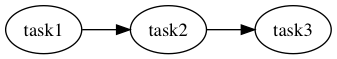
\includegraphics[width=0.5\textwidth]{./figures/workflow/tasks_flow_graph_trivialexample.png}
\end{center}
While in this case the flow chart is trivial, a real project will have a much more complicated structure that you can't remember.
See our \href{https://github.com/jdingel/DavisDingelMonrasMorales}{consumption segregation paper} for an example.

\subsection{All output is produced by tasks}

In reality, every number reported in your paper is produced by code.
Your workflow (and your replication package) therefore should produce every such number as a file in an \texttt{output} folder.
A summary statistic that appears in a sentence rather than in a table is still a code-produced number.
If you hardcode some number in your paper's \LaTeX\ file, I bet you'll forget to update it at least once (it's produced by code + human transcription and the latter is less reliable.)
I've certainly produced drafts where the same number takes different values in a paragraph and in a table because code produced the latter but not the former.

All output is produced by tasks.
Our task workflow produces the final paper.
See Patrick Ball at \href{https://www.youtube.com/watch?v=ZSunU9GQdcI&t=40m27s}{40:27}.
